\begin{frame}{[\textbf{Chapter 4}] ネットワーク上の一様な結合振動子系}
  \begin{block}{ネットワーク上の一様な結合振動子系}
  \centering
  $\displaystyle\frac{\diff\theta_{i}}{\diff t}=\sum_{j\in[N]}a_{ij}\sin(\theta_{j}-\theta_{i})$
  \begin{itemize}
    \item $\theta_{i}\in[0,2\pi)$: $i$番目の振動子の位相
    \item $a_{ij}\in\{0,1\}$: ネットワークの隣接行列の$(i,j)$成分
  \end{itemize}
  \end{block}
  % \begin{figure}
  %     \centering
  %     \includegraphics[scale=0.3]{figs/graph_mat.pdf}
  % \end{figure}
  \begin{itemize}
    \item $\bm{\theta}_{0}=(0,0,\dots,0)^{\top}$: 完全同期解、すべての位相が同じ
    \item この解はネットワークによらずに\textbf{安定}
    \begin{itemize}
        \item 密であれば必ず同期すると期待(完全同期のみが安定平衡点)
        \item どれほど``密''であれば必ず同期する?
    \end{itemize}
  \end{itemize}
  \begin{figure}
    \centering
    \includegraphics[width=\textwidth]{figs/dense_sync_ponchi.pdf}
  \end{figure}
\end{frame}

% \begin{frame}{完全同期解}
%     \begin{block}{ネットワーク上の一様な結合振動子系}
%         \centering
%         $\displaystyle\frac{\diff\theta_{i}}{\diff t}=\sum_{j\in[N]}a_{ij}\sin(\theta_{j}-\theta_{i}),\ i\in[N]$
%         \begin{itemize}
%           \item $\theta_{i}\in[0,2\pi)$: $i$番目の振動子の位相
%           \item $a_{ij}\in\{0,1\}$: ネットワークの隣接行列の$(i,j)$成分
%         \end{itemize}
%     \end{block}
% \begin{itemize}
% \item $\bm{\theta}_{0}=(0,0,\dots,0)^{\mathsf{T}}$: 完全同期解、すべての位相が同じ
% \item この解はネットワークによらずに\textbf{安定}
% \begin{itemize}
%     \item $\bm{\theta}_{0}$まわりの線形安定性解析より従う
%     \item 勾配系であることからもわかる
%     \begin{align*}
%         \frac{\diff\bm{\theta}}{\diff t} = -\frac{\partial E(\bm{\theta})}{\partial\bm{\theta}},
%         \quad E(\bm{\theta}) = -\frac{1}{2}\sum_{i,j\in[N]}a_{ij}\cos(\theta_{j}-\theta_{i})
%     \end{align*}
% \end{itemize}
% \end{itemize}
% \end{frame}

\begin{frame}{接続数(connectivity)}
\begin{block}{connectivity $\mu$}
\centering
$\displaystyle\mu = \frac{\min_{i\in[N]}\sum_{j\in[N]}a_{ij}}{N-1}$
\end{block}
\begin{itemize}
    \item $\mu$はネットワークの``密具合''を表す
    \begin{itemize}
        \item ネットワークの最小次数を規格化したもの
        \item $\mu=1$のとき全結合ネットワーク
    \end{itemize}
\end{itemize}
\begin{figure}
    \centering
    \includegraphics[width=\textwidth]{figs/mu.pdf}
\end{figure}
\end{frame}

\begin{frame}{臨界接続数(critical connectivity)}
    \centering
  $\displaystyle\frac{\diff\theta_{i}}{\diff t}=\sum_{j\in[N]}a_{ij}\sin(\theta_{j}-\theta_{i})$
    \begin{table}[htb]
        \begin{tabular}{l||l}
            完全同期以外の安定平衡点が存在 & 完全同期のみが安定 \\
            (\blue{同期しない密なネットワーク}) & (\blue{必ず同期するネットワーク}) \\\hline
          $\mu\leq0.6809\dots$ (Wiley, 2006) & $\mu=1$ (Watanabe, 1994) \\
          $\mu\leq0.6818\dots$ (Canale, 2015) & $\mu\geq0.9395\dots$ (Taylor, 2012)\\
          $\mu\leq0.6828\dots$ (Townsend, 2020) & $\mu\geq0.7929\dots$ (Ling, 2019) \\
          \cellcolor[rgb]{1.0, 0.0, 0.0} & $\mu\geq0.7889\dots$ (Lu, 2020)
        \end{tabular}
      \end{table}
\begin{itemize}
    \item $\mu_{\mathrm{c}}$: 臨界接続数、完全同期解のみが安定平衡点となる$\mu$の境界
\begin{align*}
    0.6828\dots\leq\mu_{\mathrm{c}}\leq0.7889\dots
\end{align*}
\item 本研究: \underline{\textbf{できるだけ密な同期しないネットワークを探索する}}
\end{itemize}
\end{frame}

\begin{frame}{巡回グラフ}
\begin{itemize}
\item ネットワークとして巡回グラフを考える
\begin{itemize}
    \item 巡回グラフの対応する隣接行列は巡回行列
    \item $\bm{x}\in\{0,1\}^{N-1}$: 巡回行列を生成する列
    \begin{align*}
        a_{ij}=x_{i-j\bmod N},
        \quad x_{i}=x_{N-i}
    \end{align*}
    \item 強い対称性があるおかげで諸々の値の手計算が可能
\end{itemize}
\end{itemize}
\begin{figure}
    \centering
    \includegraphics[width=0.9\textwidth]{figs/circulant_graph_matrix.pdf}
\end{figure}
\end{frame}

\begin{frame}{$p$-twisted stateと線形固有値}
    \centering
  $\displaystyle\frac{\diff\theta_{i}}{\diff t}=\sum_{j\in[N]}a_{ij}\sin(\theta_{j}-\theta_{i})$
\begin{itemize}
\item ネットワークが巡回グラフの場合、$p$-twisted stateが平衡点
\begin{align*}
\bm{\theta}_{p}=\left(0,\frac{2\pi p}{N}, \frac{4\pi p}{N},\dots, \frac{2\pi (N-1)p}{N}\right)^{\top}\quad 0\leq p\leq\left\lfloor\frac{N}{2}\right\rfloor
\end{align*}
% \begin{itemize}
% \item $p=0$は完全同期解
% \end{itemize}
\begin{figure}
    \centering
    \includegraphics[width=0.8\textwidth]{figs/twisted_state.pdf}
\end{figure}
\item $p$-twisted stateまわりのJacobian行列の固有値$\bm{\lambda}$
\begin{align*}
    \lambda_{k}=\sum_{l\in[N-1]}x_{l}\cos\left(\frac{2\pi pl}{N}\right)\left[-1+\cos\left(\frac{2\pi kl}{N}\right)\right]
\end{align*}
% \begin{itemize}
%     \item $\lambda_{0}=0$: 系の大域的回転対称性より
%     \item $\lambda_{k},k=1,\dots,N-1$の正負が$p$-twisted stateの安定性を決める
% \end{itemize}
\end{itemize}
\end{frame}

\begin{frame}{方針}
\begin{itemize}
    \item 安定平衡点を持つネットワークを色々取り替える\\
    \begin{center}
        $\Downarrow$\\
    \end{center}
    その中で$\mu$が最大となるネットワークを選ぶ
    \item \textbf{最適化問題}による定式化
    \begin{itemize}
        \item $\bm{x}\in\{0,1\}^{N-1}$ $\Longrightarrow$ \textbf{整数計画問題}
        \item 制約条件
        \begin{itemize}
            \item $\lambda_{k}<0\Leftrightarrow L^{(N,p)}\bm{x}<\bm{0}$ (安定性)
            \[
                \left[L^{(N,p)}\right]_{kl} = \cos\left(\frac{2\pi pl}{N}\right)\left[-1+\cos\left(\frac{2\pi kl}{N}\right)\right]
            \]
            \item $x_{i}=x_{N-i} \Leftrightarrow C^{(N)}\bm{x}=0$ (無向グラフ)
            \[
                \left[C^{(N)}\right]_{kl}=\delta_{k,l}-\delta_{k,N-l}
            \]
        \end{itemize}
    \end{itemize}
\end{itemize}
\end{frame}

\begin{frame}{整数計画問題としての定式化}
``$N$体の振動子を持つ系において$p$-twisted stateが安定平衡点になるようなネットワークの中で最大のconnectivityはいくらか?''
\begin{block}{整数計画問題 $(N,p)$}
$N\geq2,1\leq p\leq\lfloor N/2\rfloor$に対して
\begin{align*}
\begin{split}
\textrm{maximize} & \quad\mu=\frac{1}{N-1}\bm{1}^{\top}\bm{x}, \\
\textrm{subject to} & \quad \bm{x}\in\left\{0,1\right\}^{N-1},\\
& \quad L^{(N,p)}\bm{x}<\bm{0},\quad \red{\mathrm{[stable]}}\\
& \quad C^{(N)}\bm{x} = \bm{0}.\quad \red{\mathrm{[undirected]}}
\end{split}
\end{align*}
\end{block}
\begin{itemize}
    \item $\mu^{(N,p)}$: 各$N,p$における整数計画問題の最大値
    % \item 実行可能解が存在しない場合: $\mu^{(N,p)}=-1$
\end{itemize}    
\end{frame}

% \begin{frame}{$\mu^{(N,p)}$の数値計算}
% \begin{itemize}
%     \item 最適化ライブラリ: \texttt{JuMP}(\texttt{Julia}), \texttt{pulp}(\texttt{Python})
% \end{itemize}
% \begin{figure}
%     \centering
%     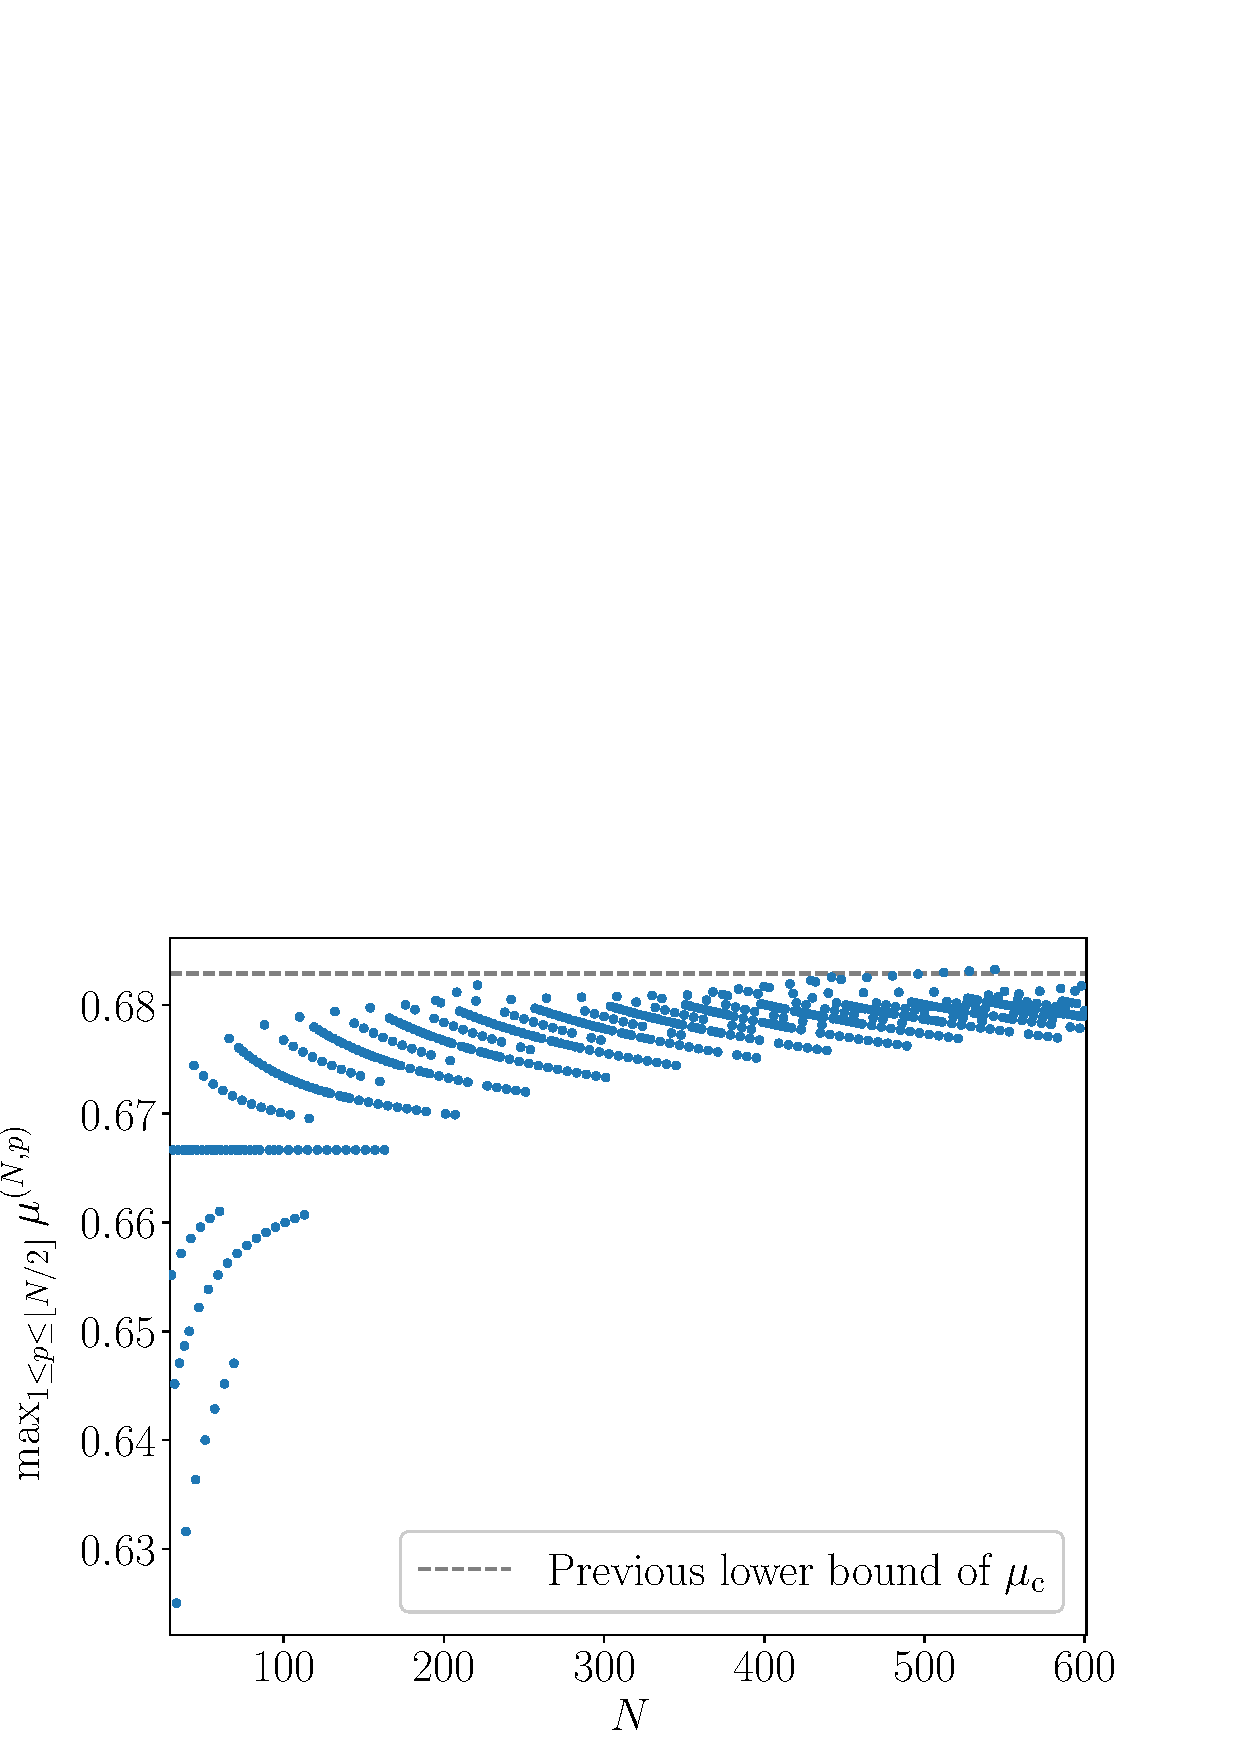
\includegraphics[width=0.9\textwidth]{figs/max_connect.pdf}
% \end{figure}
% \end{frame}

\begin{frame}{$\mu^{(N,p)}$の厳密解}
\begin{theorem}[$\mu^{(N,p)}$]
$N\geq2,1\leq p\leq\lfloor N/2\rfloor$に対して$m=\gcd(N,p),\widetilde{N}=N/m$とおく。
\begin{enumerate}
\item $\widetilde{N}=2,3,4$のとき実行可能解が存在しない。% $\mu^{(N,p)}=-1$
\item $\widetilde{N}\geq 5$のとき
\begin{align*}
    S_{k}^{(\widetilde{N})}=\sum_{l=1}^{k}\cos\left(\frac{2\pi l}{\widetilde{N}}\right)\left[-1+\cos\left(\frac{2\pi l}{\widetilde{N}}\right)\right]
\end{align*}
とし、$k_{\mathrm{c}}^{(\widetilde{N})}$を$S_{k}^{(\widetilde{N})}\geq0$なる最小の$k$と定義する。このとき、
\begin{align*}
    \mu^{(N,p)}=\frac{m(2k_{\mathrm{c}}-1)-1-2\lfloor mS_{k_{\mathrm{c}}-1}/(S_{k_{\mathrm{c}}}-S_{k_{\mathrm{c}}-1})\rfloor}{N-1}
\end{align*}
\end{enumerate}
\end{theorem}
\end{frame}

\begin{frame}{$\mu_{\mathrm{c}}$の下限}
\begin{theorem}[$\sup \mu^{(N,p)}$]
\begin{align*}
    &\sup\left\{\mu^{(N,p)} \mathrel{}\middle|\mathrel{} 1\leq p\leq \lfloor N/2\rfloor, N\geq2\right\}\\
    =&\lim_{m\to\infty}\mu^{(19m,m)}\\
    =&\frac{11}{19}-\frac{2}{19}\frac{\sum_{l=1}^{5}\left[-\cos\left(\frac{2\pi l}{19}\right)+\cos^{2}\left(\frac{2\pi l}{19}\right)\right]}{-\cos\left(\frac{12\pi}{19}\right)+\cos^{2}\left(\frac{12\pi}{19}\right)}=\red{0.683875\dots}
\end{align*}
\end{theorem}
\begin{itemize}
\item $\mu\leq 0.6838\dots$なるネットワークが存在して、完全同期解以外の安定平衡点が存在する。
\begin{align*}
    0.6838\dots\leq\mu_{\mathrm{c}}\leq0.7889\dots
\end{align*}
\end{itemize}
\end{frame}

\begin{frame}{まとめと展望}
    \centering
  $\displaystyle\frac{\diff\theta_{i}}{\diff t}=\sum_{j\in[N]}a_{ij}\sin(\theta_{j}-\theta_{i})$
    \begin{table}[htb]
        \begin{tabular}{l||l}
          完全同期以外の安定平衡点が存在 & 完全同期のみが安定 \\
          (\blue{同期しない密なネットワーク}) & (\blue{必ず同期するネットワーク}) \\\hline
          $\mu\leq0.6809\dots$ (Wiley, 2006) & $\mu=1$ (Watanabe, 1994) \\
          $\mu\leq0.6818\dots$ (Canale, 2015) & $\mu\geq0.9395\dots$ (Taylor, 2012)\\
          $\mu\leq0.6828\dots$ (Townsend, 2020) & $\mu\geq0.7929\dots$ (Ling, 2019) \\
          \red{$\mu\leq0.6838\dots$ (Yoneda, 2021)} & $\mu\geq0.7889\dots$ (Lu, 2020) \\ \hdashline \hdashline
          \green{$\mu\leq0.6875$ (Canale, 2022)} & \green{$\mu\geq0.75$ (Townsend, 2021)}
        \end{tabular}
      \end{table}
\begin{itemize}
    \item \textbf{$\mu_{\mathrm{c}}$の下からの評価について}
    \begin{itemize}
        \item 巡回グラフにおける他の平衡点? 他のネットワーク?
    \end{itemize}
\end{itemize}
\end{frame}